  \chapter{Tecnologias utilizadas na construção de chatbots}
  
  \section{Ferramentas e Frameworks}
  \subsection{Chatfuel}
  Chatfuel é o \textit{framework} mais utilizado na criação de \textit{bots}. Através de uma plataforma totalmente online, o serviço permite a criação de \textit{chatbots} através de um painel. Segundo dados da própria companhia, cerca de 46\% dos \textit{chatbots} desenvolvidos para o Facebook Messenger\footnote{Disponível em https://chatfuel.com/} são criados com a plataforma.
  
  Com o Chatfuel é possível criar \textit{bots} baseados em regras ou com inteligência baseada em palavras-chave, com treinamento feito diretamente pelo painel de administração.
  
  O plano gratuito permite até 1000 usuários assinantes e exibe uma propaganda no \textit{chatbot} indicando que ele foi desenvolvido com a ferramenta.
  
  \subsection{Botpress}
   O Botpress é um \emph{framework} \emph{open-source} de criação de bots desenvolvido em JavasScript que contém toda a infraestrutura necessária para produzir chatbot sem a necessidade de escrever muito código. Executado com o Node.js e disponível no repositório do NPM, o Botpress é focado na simplicidade e na intuitividade para o desenvolvimento de \textit{chatbots}, oferecendo um painel interativo para criação de fluxos de conversa e um simulador para testes, o que permite a construção de um \textit{chatbot} completo de forma bem mais rápida. Além disso, também é possível adicionar novas funcionalidades através da instalação de módulos.
  
   Os módulos do Botpress são componentes que não fazem parte do Core principal do \textit{framework}, mas que podem ser instalados para adicionar novas funcionalidades. Os módulos se dividem em três categorias: módulos de canais, módulos de skills e módulos funcionais.
  
  Os módulos de canais são os componentes que permitem com que o \textit{chatbot} envie e receba mensagens de uma plataforma específica, como Facebook Messenger, Telegram, etc. Para que isso aconteça, o Botpress Core implementa um mecanismo de enfileiramento que processa as mensagens que chegam e que saem, sequencialmente. Caso haja alguma falha nesse processo (um erro de envio, por exemplo) é feita uma nova tentativa de processamento da mensagem, antes de gerar um erro.
  
  Skills são componentes que podem ser incluídos nos fluxos de conversa. Dessa forma, os módulos de skills são aqueles módulos que instalam tais componentes. Um exemplo de módulo de skill, por exemplo, é o \textbf{múltipla escolha}.
  
  \begin{figure}[h!]
  	\begin{center}
  		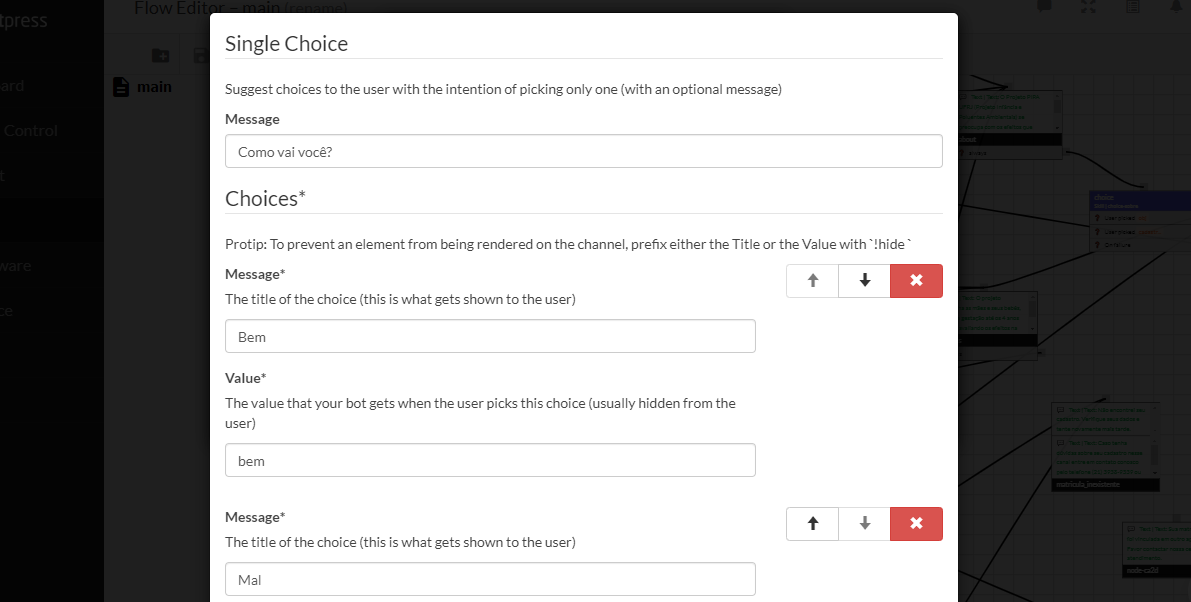
\includegraphics[width=0.95\linewidth]{images/choice.png}
  		\caption{\textit{Choice} - Componente de respostas através de opções de múltipla escolha}
  		\label{fig:choice}
  	\end{center}
  \end{figure}
  
  Diferentemente dos módulos de skill e de canais, que estendem as funcionalidades já existentes do Botpress, os módulos funcionais são aqueles que incluem funcionalidades novas. Um exemplo de módulo funcional é o HITL (Human in the loop). Com esse módulo, é possível pausar o \textit{chatbot} em conversas específicas, permitindo um humano interagir com o usuário diretamente pelo painel, como mostrado na figura \ref{fig:hitl}.
  
  \begin{figure}[h!]
  	\begin{center}
  		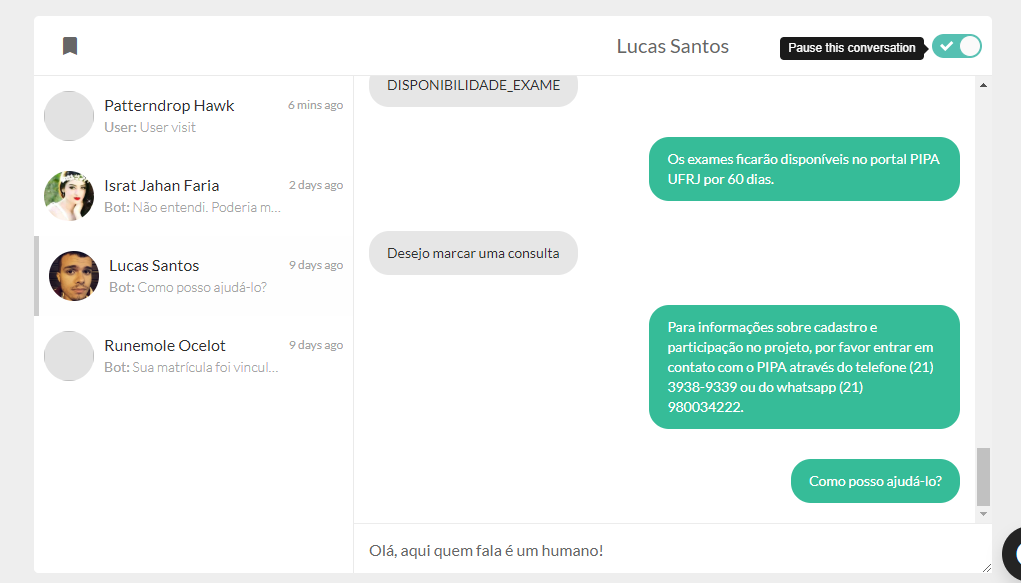
\includegraphics[width=0.95\linewidth]{images/hitl.png}
  		\caption{\textit{HITL} - Interface de troca de mensagens no painel do Botpress}
  		\label{fig:hitl}
  	\end{center}
  \end{figure}
  
  Por fim, o Botpress também permite criar \emph{actions} (ações). Essas ações são trechos de código escritos em JavaScript que, diferente dos módulos, só são executadas quando invocados por algum bloco do fluxo da conversa, como na figura \ref{fig:action}.
  
  \begin{figure}[h!]
  	\begin{center}
  		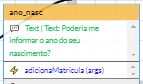
\includegraphics[width=0.35\linewidth]{images/action.png}
  		\caption{\textit{Actions} - Bloco com uma função javascript que é executada após o envio da mensagem.}
  		\label{fig:action}
  	\end{center}
  \end{figure}
  
  
  \section{Canais}
  \subsection{Facebook Messenger}
  É o aplicativo de mensagens desenvolvido originalmente para ser a plataforma de chat do Facebook. Com ele, os usuários podem se comunicar com outros usuários da plataforma através de textos, chamada de voz ou vídeo e também compartilhar diversos tipos de mídia e arquivos.% Dentre os tipos de mídia, é possível compartilhar fotos, vídeos, figurinhas, áudios e até mesmo outros formatos de arquivos em geral (acessados via download).
  
  Em 2016 o Facebook anunciou uma plataforma de bots para o Messenger que recebe constantes melhorias desde então. Hoje, é possível que usuários façam \textbf{assinaturas} para receber conteúdos diretamente dos bots que ele conversa. Por padrão, os bots apenas respondem a mensagens de usuários mas com uma assinatura é possível com que o bot proativamente envie a mensagem.
  
  %Além disso, é possível gerar QR Codes que podem ser lidos pela câmera do Facebook Messenger que levam os usuários diretamente para uma janela de conversa com o bot.
  \subsection{Telegram}
  É um aplicativo de troca de mensagens multiplataforma, podendo ser acessado através de smartphones, computadores, ou pela interface web. Assim como o Messenger, é possível compartilhar arquivos de mídia com outros usuários. Por sua infraestrutura ser baseada em nuvem, é possível acessar as mídias de uma conversa de qualquer lugar. Além disso, todos os clients do Telegram são opensource, e o serviço disponibiliza APIs para desenvolvedores criarem suas aplicações.
  
  No Telegram, bots são um tipo especial de conta que não requer um número telefônico para ser criado. Os usuários interagem enviando mensagens e comandos pela conversa ou adicionando o bot a grupos. As mensagens são armazenadas nos servidores do Telegram até que o serviço que controle o bot leia e processe as mensagens. Os bots não podem enviar mensagens diretamente para qualquer usuário; é preciso que o usuário inicie uma conversa ou que ele seja adicionado a um grupo.
  
  
  \subsection{Slack}
  Slack é uma ferramenta colaborativa que tem como objetivo reunir pessoas, informações e as ferramentas certas para desenvolver algum tipo de trabalho. É largamente usado como ferramenta de comunicação em empresas.
  
  Na plataforma, bots são um tipo de aplicativo que interage com o usuário através da conversação. Ele recebe exatamente os mesmos acessos que uma aplicação comum do Slack (inclusive, ao adicionarmos um bot, adicionamos uma integração - que é limitado pelo plano gratuito do Slack), com diferença que ele se torna um usuário como um outro qualquer do espaço colaborativo. É possível mencioná-lo em conversas, é possível mandar mensagens diretas, enviar arquivos e adicionar em grupos. Além disso, bots tem permissões para abrir uma nova conversa com algum usuário caso seja programado para isso.
  %\subsection{WhatsApp}
  
  \section{Provedores de inteligência artificial e NLP}
  \subsection{Wit.ai}
  Wit.ai é um provedor de inteligencia artificial e processamento de linguagem natural gratuito criado pelo Facebook para ser integrado a diversos tipos de aplicações de software como aplicativos, wearables e bots\footnote{https://wit.ai/}. Suporta cerca de 50 linguagens diferentes.
  \subsection{IBM Watson}
  IBM Watson é uma suíte completa de ferramentas voltadas para inteligência artificial. Desenvolvida pela IBM, tem como principal destaque a precisão na detecção de intents mesmo com uma base de treino pequena. Com o Watson Assistant é possível desenvolver gratuitamente um \textit{chatbot} sendo limitado a 10.000 chamadas de API por mês\footnote{https://www.ibm.com/watson/how-to-build-a-chatbot}.
  \subsection{LUIS.ai}
  É um serviço baseado em machine learning criado pela Microsoft focado em fornecer processamento de linguagem natural para bots, apps e dispositivos IoT. Desenhado para reconhecer informações de valor em mensagens de texto, o LUIS.ai é capaz de se integrar a outras ferramentas que compõem a suíte de aplicativos do Azure, como o Azure Bot Service\footnote{https://www.luis.ai/home}. Atualmente suporta cerca de 13 linguagens diferentes\footnote{https://docs.microsoft.com/pt-br/azure/cognitive-services/luis/luis-language-support}.
  %\section{outras coisas????}
  
  %Colocar tudo que você usou. Veja como a Andrea fez.
  